\section{Perfilado de código}

El perfilado de código (\textit{profiling}) es el proceso de medir el comportamiento
de un programa en ejecución con el objetivo de identificar dónde se concentra el
costo computacional y de memoria.
A diferencia del análisis estático, el perfilado opera sobre la ejecución real del
programa, capturando métricas como tiempo por función, contadores de hardware del
procesador, comportamiento de la jerarquía de caché y consumo dinámico de memoria.
Esto permite construir evidencia empírica que justifica las decisiones de optimización
y sirve de línea base para comparar implementaciones alternativas.

El script \texttt{bench\_profiling.sh} orquesta seis técnicas de perfilado
complementarias sobre la implementación secuencial de multiplicación de matrices,
para los tamaños $N \in \{128, 256, 512, 1024\}$.
Cada técnica responde una pregunta distinta: cuánto tiempo tarda, en qué función
se acumula ese tiempo, qué eventos de hardware ocurren, cómo se comporta la
jerarquía de caché y cuánta memoria dinámica se consume.
Los resultados de todas las herramientas se consolidan en un archivo CSV
(\texttt{data\_profiling.csv}) que sirve de entrada al generador de reportes.


\subsection{gprof: perfilado por instrumentación del compilador}

\texttt{gprof} es una herramienta de perfilado basada en instrumentación generada
en tiempo de compilación~\parencite{graham1982gprof}.
El binario \texttt{mul\_seq\_gprof} se compila con las flags \texttt{-pg} y
\texttt{-fno-inline}:

\begin{itemize}
    \item \textbf{\texttt{-pg}}: instruye al compilador para insertar una llamada a
        la función \texttt{mcount()} al inicio de cada función del programa.
        Durante la ejecución, estas llamadas actualizan en tiempo real los
        contadores de frecuencia de invocación y los acumuladores de tiempo en un
        archivo binario llamado \texttt{gmon.out}.
    \item \textbf{\texttt{-fno-inline}}: impide que el compilador reemplace el cuerpo
        de las funciones directamente en sus sitios de llamada (\textit{inlining}).
        
\end{itemize}

El reporte que produce \texttt{gprof} tiene dos partes principales:

\begin{itemize}
    \item \textbf{Flat profile}: lista cada función con el porcentaje del tiempo total
        que le corresponde, los segundos acumulados, el número de veces que fue
        invocada y el tiempo promedio por llamada.
        Este perfil responde directamente la pregunta \textit{``¿en qué función
        pasa el programa la mayor parte del tiempo?''}.
    \item \textbf{Call graph}: muestra la jerarquía de llamadas entre funciones y
        cuánto tiempo se propaga desde cada función hija hacia su función padre.
        Es útil para distinguir si una función es costosa por su propia lógica o
        porque invoca a subfunciones costosas.
\end{itemize}

La limitación de \texttt{gprof} es que su medición del tiempo se basa
en muestreo estadístico del contador de programa (\textit{program counter}) con
una resolución de aproximadamente 10\,ms.
Para programas de corta duración o con alta granularidad de funciones los
porcentajes pueden ser estadísticamente ruidosos.
Además, al requerir recompilación con instrumentación, el binario perfilado no es
idéntico al binario de producción, lo que puede alterar el comportamiento de caché
y el layout de código.


\subsection{perf stat: contadores de hardware de la PMU}

\texttt{perf stat} accede directamente a la \textit{Performance Monitoring Unit}
(PMU), un conjunto de registros físicos presentes en el procesador
diseñados específicamente para contar eventos de hardware con un overhead
mínimo sobre el programa medido.

El conjunto de eventos medidos cubre cuatro categorías de cuello de botella típicos
en el contexto de la multiplicación de matrices:

\paragraph{Throughput del pipeline.}
Los eventos \texttt{cycles} e \texttt{instructions} permiten calcular el
\textit{Instructions Per Cycle} (IPC):
\begin{equation}
    \text{IPC} = \frac{\text{instructions}}{\text{cycles}}.
\end{equation}
Un IPC cercano a 1 indica que por cada ciclo de reloj el procesador completa en
promedio una instrucción.
Valores menores a 1 señalan que el pipeline sufre \textit{stalls} frecuentes,
generalmente por esperas de memoria.
Valores mayores a 2 indican que el procesador está emitiendo múltiples
instrucciones por ciclo de forma efectiva gracias al paralelismo a nivel de
instrucción (ILP).

\paragraph{Caché de último nivel (LLC).}
Los eventos \texttt{cache-references} y \texttt{cache-misses} miden la presión
sobre la LLC (\textit{Last Level Cache}).
La tasa de fallo
\begin{equation}
    \text{LLC miss rate} = \frac{\text{cache-misses}}{\text{cache-references}} \times 100\%
\end{equation}
indica qué fracción de los accesos a la LLC no encontró el dato solicitado y tuvo
que recurrir a la memoria principal (DRAM).
En multiplicación de matrices, para tamaños grandes de $N$, las tres matrices no
caben simultáneamente en LLC y esta tasa escala drásticamente, siendo el principal
responsable de la degradación del rendimiento con respecto al pico teórico del
procesador.

\paragraph{Caché L1 de datos (L1-D).}
Los eventos \texttt{L1-dcache-loads} y \texttt{L1-dcache-load-misses} miden la
localidad efectiva del acceso a datos en el nivel de caché más cercano al
procesador.
La tasa de fallo en L1-D es el indicador más sensible al orden de los bucles en
el algoritmo: el orden $i$-$j$-$k$ produce accesos no contiguos a la
columna \texttt{matrix2[k][j]}, penalizando directamente este contador.

\paragraph{Translation Lookaside Buffer (TLB).}
Los eventos \texttt{dTLB-loads} y \texttt{dTLB-load-misses} miden el costo
de la traducción de direcciones virtuales a físicas.
El TLB es una caché especializada de entradas de la tabla de páginas del sistema
operativo.
Cuando se trabaja con matrices grandes cuyos elementos están distribuidos en
muchas páginas de memoria virtual, los fallos de TLB agregan latencia adicional
independiente de la jerarquía de caché de datos.
Esta métrica permite separar si la degradación de rendimiento se debe a presión
de caché o a presión de TLB.

\paragraph{Predictor de saltos.}
Los eventos \texttt{branch-instructions} y \texttt{branch-misses} cuantifican la
efectividad del predictor de saltos del procesador.
En un algoritmo de multiplicación de matrices con bucles perfectamente regulares
se espera una tasa de fallo del predictor cercana a cero, ya que todos los saltos
son altamente predecibles.
Un valor elevado sería indicativo de lógica condicional inesperada en el código
o de fallos en la vectorización automática.

\subsection{perf mem: perfilado de accesos a la jerarquía de memoria}

\texttt{perf mem} es una extensión especializada de \texttt{perf} diseñada
específicamente para analizar el comportamiento de los accesos a memoria,
distinguiendo en qué nivel de la jerarquía fue satisfecho cada acceso
(\textit{memory hierarchy attribution}).
Mientras que \texttt{perf stat} reporta tasas de fallo de caché como totales
globales y \texttt{perf record} localiza funciones costosas, \texttt{perf mem}
responde una pregunta más precisa: \textit{``¿desde qué nivel de la jerarquía
de memoria se están sirviendo los accesos de carga del programa?''}

El script ejecuta la herramienta en dos fases:

\begin{itemize}
    \item \textbf{\texttt{perf mem record}}: captura muestras de eventos de
        acceso a memoria mediante los registros PEBS (\textit{Precise Event
        Based Sampling}) disponibles en procesadores Intel, o su equivalente
        en AMD.
        A diferencia del muestreo por ciclos de \texttt{perf record}, PEBS
        captura el evento en el ciclo exacto en que ocurre la instrucción de
        carga, lo que elimina el \textit{skid} (desplazamiento entre el evento
        real y la muestra registrada) y permite atribuir con precisión cada
        acceso a la instrucción que lo causó.
    \item \textbf{\texttt{perf mem report --sort=mem}}: formatea el reporte
        agrupando las muestras por tipo de acceso a memoria.
        La opción \texttt{-t load} restringe el análisis a operaciones de
        lectura, que son las dominantes en la multiplicación de matrices donde
        los elementos de las matrices de entrada se leen repetidamente.
        La opción \texttt{--sort=mem} agrupa los resultados por nivel de la
        jerarquía de memoria que sirvió el acceso.
\end{itemize}

El reporte resultante distribuye el porcentaje de accesos de carga entre los
siguientes niveles de la jerarquía:

\begin{itemize}
    \item \textbf{L1 hit}: acceso satisfecho por la caché de datos de nivel 1.
        Representa el caso ideal: latencia de 4--5 ciclos.
    \item \textbf{L2 hit}: acceso satisfecho por la caché de nivel 2.
        Latencia típica de 12--15 ciclos.
    \item \textbf{L3 hit} (LLC hit): acceso satisfecho por la caché de último
        nivel.
        Latencia típica de 30--40 ciclos según la arquitectura.
    \item \textbf{LFB hit} (\textit{Line Fill Buffer}): acceso satisfecho por
        el buffer de relleno de línea, una estructura interna del procesador que
        almacena temporalmente líneas de caché en tránsito entre niveles.
        Un porcentaje alto de LFB hits indica alta presión de ancho de banda
        entre L1 y L2.
    \item \textbf{RAM hit}: acceso que no fue satisfecho por ningún nivel de
        caché y tuvo que recurrir a la memoria principal (DRAM).
        Latencia de 100--300 ciclos, dependiendo del acceso NUMA y la
        contención del bus de memoria.
\end{itemize}

La utilidad de \texttt{perf mem} en el contexto de la multiplicación de matrices
reside en cuantificar la distribución efectiva de latencias: para
$N = 128$ se espera que la mayoría de accesos sean L1 o L2 hits porque las
matrices caben en los niveles superiores de caché, mientras que para $N = 1024$
el porcentaje de RAM hits debe escalar significativamente, ya que las tres
matrices ocupan aproximadamente $3 \times 1024^2 \times 4 \approx 12$\,MB,
superando la capacidad típica de L2 (256\,KB--1\,MB) y presionando la LLC.
Esta distribución complementa los miss rates de \texttt{perf stat} con
información cualitativa sobre el \textit{mix} de latencias que experimenta el
programa en cada tamaño de problema.

La diferencia clave con \texttt{perf stat} es que \texttt{perf mem} proporciona
una \textbf{vista por muestra y por nivel}, no solo contadores agregados.
Mientras que \texttt{perf stat} indica cuántos fallos de L1 ocurrieron en total,
\texttt{perf mem} indica qué fracción del tiempo el procesador estuvo esperando
datos de L2, L3 o RAM, lo cual es directamente proporcional al impacto en el
tiempo de ejecución.

\subsection{perf record: muestreo basado en interrupciones de hardware}

Mientras que \texttt{perf stat} reporta totales globales, \texttt{perf record}
ofrece una vista espacial de dónde en el código ocurren los eventos de CPU.
El script lo ejecuta con las opciones \texttt{-F~999} y \texttt{-g}:

\begin{itemize}
    \item \textbf{\texttt{-F 999}}: configura la frecuencia de muestreo en
        aproximadamente 999 muestras por segundo.
        Cada muestra se captura mediante una interrupción de hardware generada por
        la PMU cuando el contador de ciclos alcanza un umbral predefinido.
    \item \textbf{\texttt{-g}}: captura el \textit{call stack} completo en el
        momento de cada interrupción, lo que permite reconstruir no solo qué
        función estaba activa sino toda la cadena de llamadas que llegó hasta ella.
\end{itemize}

El resultado es un histograma que responde la pregunta: \textit{``¿qué fracción
del tiempo de CPU estuvo el procesador ejecutando instrucciones de cada
función?''}
Esta métrica es equivalente en concepto al flat profile de \texttt{gprof}, pero
con dos ventajas clave: \texttt{perf record} no requiere recompilar el programa y
mide el binario en sus condiciones reales de optimización \texttt{-O2}, incluyendo
el código de las bibliotecas del sistema como la libc.
Esto lo convierte en el perfilador de referencia para confirmar los resultados de
\texttt{gprof} en condiciones de producción.


\subsection{Valgrind Massif: perfilado de uso del heap}

Massif es una herramienta del framework Valgrind que ejecuta el programa dentro de
una máquina virtual de instrumentación binaria e intercepta todas las llamadas a
las funciones de gestión de memoria dinámica (\texttt{malloc}, \texttt{calloc},
\texttt{realloc}, \texttt{free} y sus equivalentes en C++) sin necesidad de
modificar el código fuente.

Durante la ejecución, Massif registra periódicamente \textit{snapshots} del estado
del heap, cada uno compuesto por:

\begin{itemize}
    \item \textbf{Total bytes}: memoria total reservada en ese instante.
    \item \textbf{Useful heap bytes}: memoria correspondiente a bloques solicitados
        explícitamente por el programa.
    \item \textbf{Extra heap bytes}: overhead interno del gestor de memoria
        (metadata de los bloques, alineación y fragmentación interna).
\end{itemize}

La herramienta \texttt{ms\_print} formatea estos snapshots en un reporte textual
con una gráfica ASCII de la evolución temporal del heap, identificando el snapshot
de pico y la pila de llamadas que originó las reservas de mayor tamaño.

El valor que el script extrae y almacena en el CSV es el \textbf{peak heap en MB},
que representa el máximo uso de memoria dinámica durante toda la ejecución.
Para la multiplicación de matrices con representación \textit{array de punteros}
(\texttt{int~**}), el modelo teórico de este valor es:
\begin{equation}
    M_{\text{teórico}} = \frac{3 \cdot \left(N^2 \cdot 4 + N \cdot 8\right)}{1024^2}
    \;\text{MB},
\end{equation}
donde $N^2 \cdot 4$ son los bytes de datos enteros de cada matriz y $N \cdot 8$
son los bytes del array de punteros a filas en una arquitectura de 64 bits.
La diferencia entre el valor medido por Massif y este modelo teórico cuantifica el
overhead de fragmentación interna del asignador de memoria del sistema.


\subsection{Valgrind Cachegrind: simulación de la jerarquía de caché}

Cachegrind es una herramienta del framework Valgrind que, a diferencia de
\texttt{perf stat}, no utiliza contadores de hardware reales sino que
\textbf{simula} la jerarquía de caché del procesador mediante instrumentación
a nivel de instrucción~\parencite{nethercote2007valgrind}.
Cada operación de carga y almacenamiento del programa es interceptada y procesada
por un modelo de caché configurable que reproduce la estructura de caché L1, L2
y LLC del sistema.

La métrica fundamental que produce Cachegrind es \textbf{Ir}
(\textit{Instruction References}): el conteo exacto y determinístico de
instrucciones ejecutadas durante toda la corrida.
A diferencia de los contadores de hardware, este valor es completamente
reproducible entre ejecuciones, ya que no depende del estado transitorio del
hardware.

El reporte generado por \texttt{cg\_annotate} presenta tres niveles de
granularidad:

\begin{itemize}
    \item \textbf{Program totals}: instrucciones totales de todo el programa,
        incluyendo bibliotecas del sistema.
    \item \textbf{Function summary}: distribución porcentual de instrucciones por
        función, ordenadas de mayor a menor costo.
        Permite identificar el hotspot dominante con precisión absoluta.
    \item \textbf{Annotated source}: distribución de instrucciones línea por
        línea dentro del código fuente.
        Es el nivel más granular: identifica exactamente qué sentencias del código
        son las más costosas en términos de instrucciones ejecutadas, permitiendo
        correlacionar el costo con el acceso específico a elementos de las matrices.
\end{itemize}

La principal diferencia con \texttt{perf stat} es su naturaleza determinística:
Cachegrind siempre produce el mismo conteo de instrucciones para una entrada dada,
mientras que los contadores de hardware presentan variación estadística entre
corridas por efectos del entorno.
Sin embargo, Cachegrind ejecuta el programa entre 20 y 100 veces más lento que
su velocidad normal debido al overhead de la instrumentación binaria, por lo que
sus tiempos de ejecución no son representativos del rendimiento real.


\subsection{Visión de conjunto y complementariedad}

Las seis técnicas de perfilado del script cubren distintas dimensiones del
comportamiento del programa, ninguna de ellas por sí sola es suficiente para
construir un diagnóstico completo.
La Tabla~\ref{tab:profiling_tools} resume la complementariedad entre herramientas.

\begin{table}[H]
\centering
\caption{Herramientas de perfilado utilizadas, su tipo de medición y su limitación principal}
\label{tab:profiling_tools}
\begin{tabular}{p{2.8cm}p{3.0cm}p{4.5cm}p{3.5cm}}
\toprule
\textbf{Herramienta} & \textbf{Tipo} & \textbf{Pregunta que responde} & \textbf{Limitación principal} \\
\midrule
Temporización    & Wall-clock estadístico    & ¿Cuánto tarda? ¿Es estable? & Sin resolución por función \\
\texttt{gprof}   & Instrumentación compilador & ¿Qué función consume más CPU? & Binario modificado; resolución de 10\,ms \\
\texttt{perf stat} & Contadores hardware (PMU) & ¿Qué eventos de hardware ocurren? & Solo totales globales \\
\texttt{perf mem}    & Muestreo PEBS de cargas   & ¿Desde qué nivel de memoria se sirven los accesos? & Solo procesadores con soporte PEBS \\
\texttt{perf record} & Muestreo por interrupciones & ¿Dónde está el CPU la mayor parte del tiempo? & Resolución de $\sim$1\,ms \\
Valgrind Massif  & Intercepción de heap       & ¿Cuánta memoria dinámica se usa? & 5--30$\times$ overhead \\
Valgrind Cachegrind & Simulación de caché     & ¿Qué instrucciones son más costosas? & Modelo aproximado; 20--100$\times$ overhead \\
\bottomrule
\end{tabular}
\end{table}


%================================
\subsection{Resultados del perfilado}
\label{sec:Resultados del perfilado}

La Tabla~\ref{tab:seq_profiling} consolida los resultados de las seis técnicas de perfilado aplicadas a la multiplicación de matrices clásica para tamaños crecientes, $N \in \{128, 256, 512, 1024\}$. El uso de distintas herramientas permite identificar con precisión el origen de las limitaciones de rendimiento observadas. Algo que aclarar sobre el uso de distintos tamaños de matrices es que es útil para el perfilado de memoria y no para el de CPU sabiendo que con distintos tamaños de matrices se pueden identificar distintos cuellos de botella relacionados con la jerarquía de memoria, mientras que el perfilado de CPU se enfoca en identificar el hotspot dominante, que es el mismo para todos los tamaños. Por eso, aunque se ejecutaron las seis técnicas para los cuatro tamaños, el análisis del hotspot se centra exclusivamente en $N=1024$, que es el caso más representativo del comportamiento real del programa en producción.

\textbf{Nota}: El perfilado se hizo en la maquina 1.

\begin{table}[H]
\centering
\caption{Caracterización de la implementación secuencial de multiplicación de matrices}
\label{tab:seq_profiling}
\resizebox{\textwidth}{!}{%
\begin{tabular}{rrrrrrrrrr}
\toprule
$N$ & Time mean (ms) & Std (ms) & GFLOPS & IPC & Cache Miss \% & L1 Miss \% & dTLB Miss \% & Branch Miss \% & Peak Heap (MB) \\
\midrule
128  & 0.750   & 0.008 & 5.5924 & 5.6341 & 1.44 & 2.20  & 0.0000 & 0.0000 & 0.194  \\
256  & 6.014   & 0.012 & 5.5794 & 3.4133 & 0.42 & 1.88  & 1.8833 & 0.0064 & 0.760  \\
512  & 79.801  & 0.165 & 3.3638 & 2.8634 & 0.04 & 19.78 & 0.0035 & 0.1952 & 3.016  \\
1024 & 702.284 & 5.780 & 3.0579 & 2.6175 & 1.81 & 29.74 & 0.0019 & 0.0956 & 12.027 \\
\bottomrule
\end{tabular}%
}
\end{table}

\subsubsection{Localización del hotspot}

Las herramientas de perfilado coinciden en señalar la función de multiplicación como la única fuente relevante de cómputo. El reporte de gprof le atribuye el 100\% del tiempo de ejecución, mientras que perf record indica que para $N=1024$ esta función concentra el 98.28\% de la actividad en el procesador, dejando apenas un 1.7\% restante a rutinas del programa como la inicialización y el llenado de matrices. Valgrind Cachegrind refuerza este resultado al asociarle el 98.5\% de las referencias de instrucción contabilizadas. Con esto podemos decir que todo el peso computacional recae sobre los tres bucles anidados del algoritmo, y cualquier optimización debe dirigirse exclusivamente a esa región.

\begin{figure}[H]
\centering
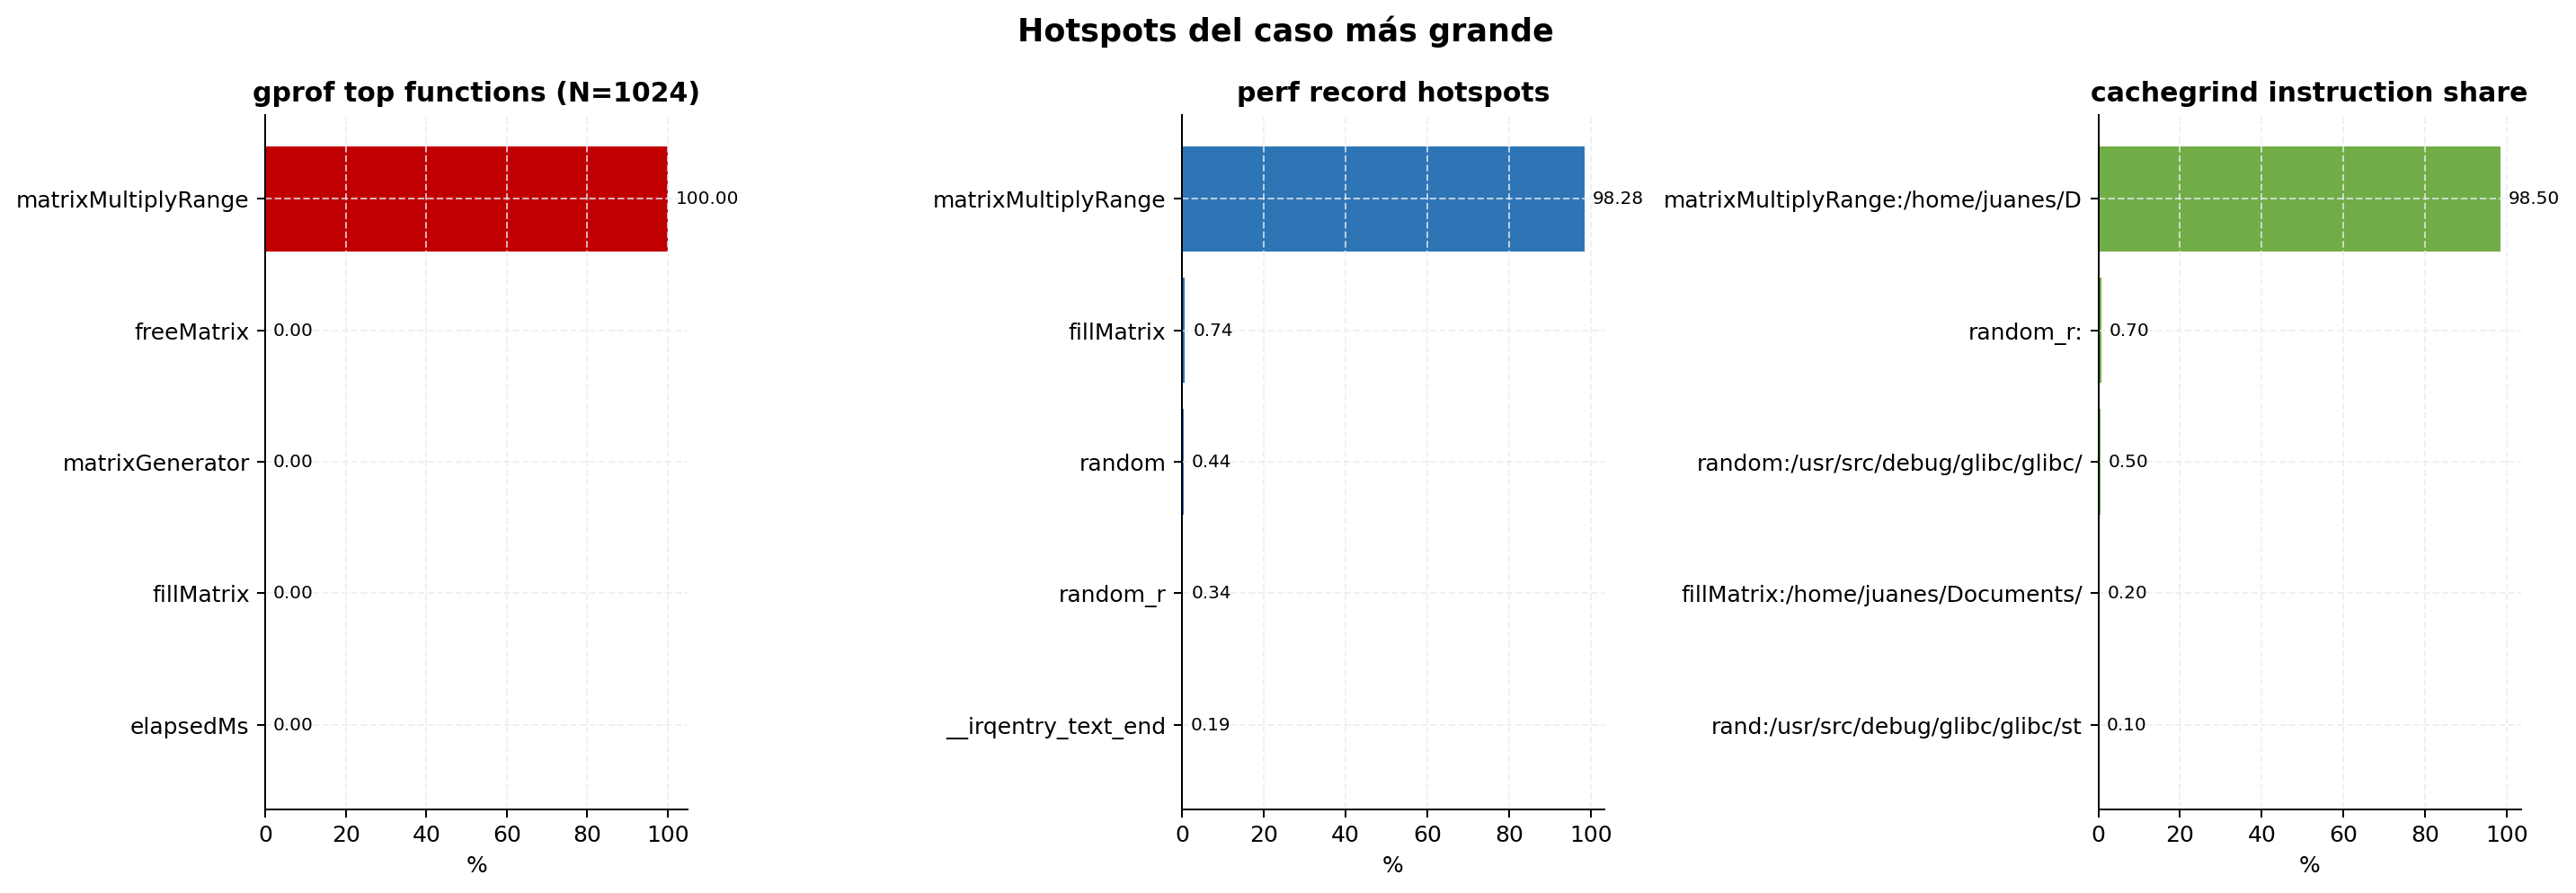
\includegraphics[width=1\textwidth]{images/profiling/05_hotspots_largest_n.png}
\caption{Distribución de tiempo e instrucciones en el hotspot principal durante el perfilado para el tamaño mayor ($N=1024$).}
\label{fig:prof_hotspot}
\end{figure}

\subsubsection{Limitaciones de hardware}

Las métricas recopiladas con perf stat muestran una caída sostenida del rendimiento a medida que crece el tamaño de la matriz, pasando de 5.53 GFLOPS para $N=128$ hasta 3.07 GFLOPS para $N=1024$.

\begin{figure}[H]
\centering
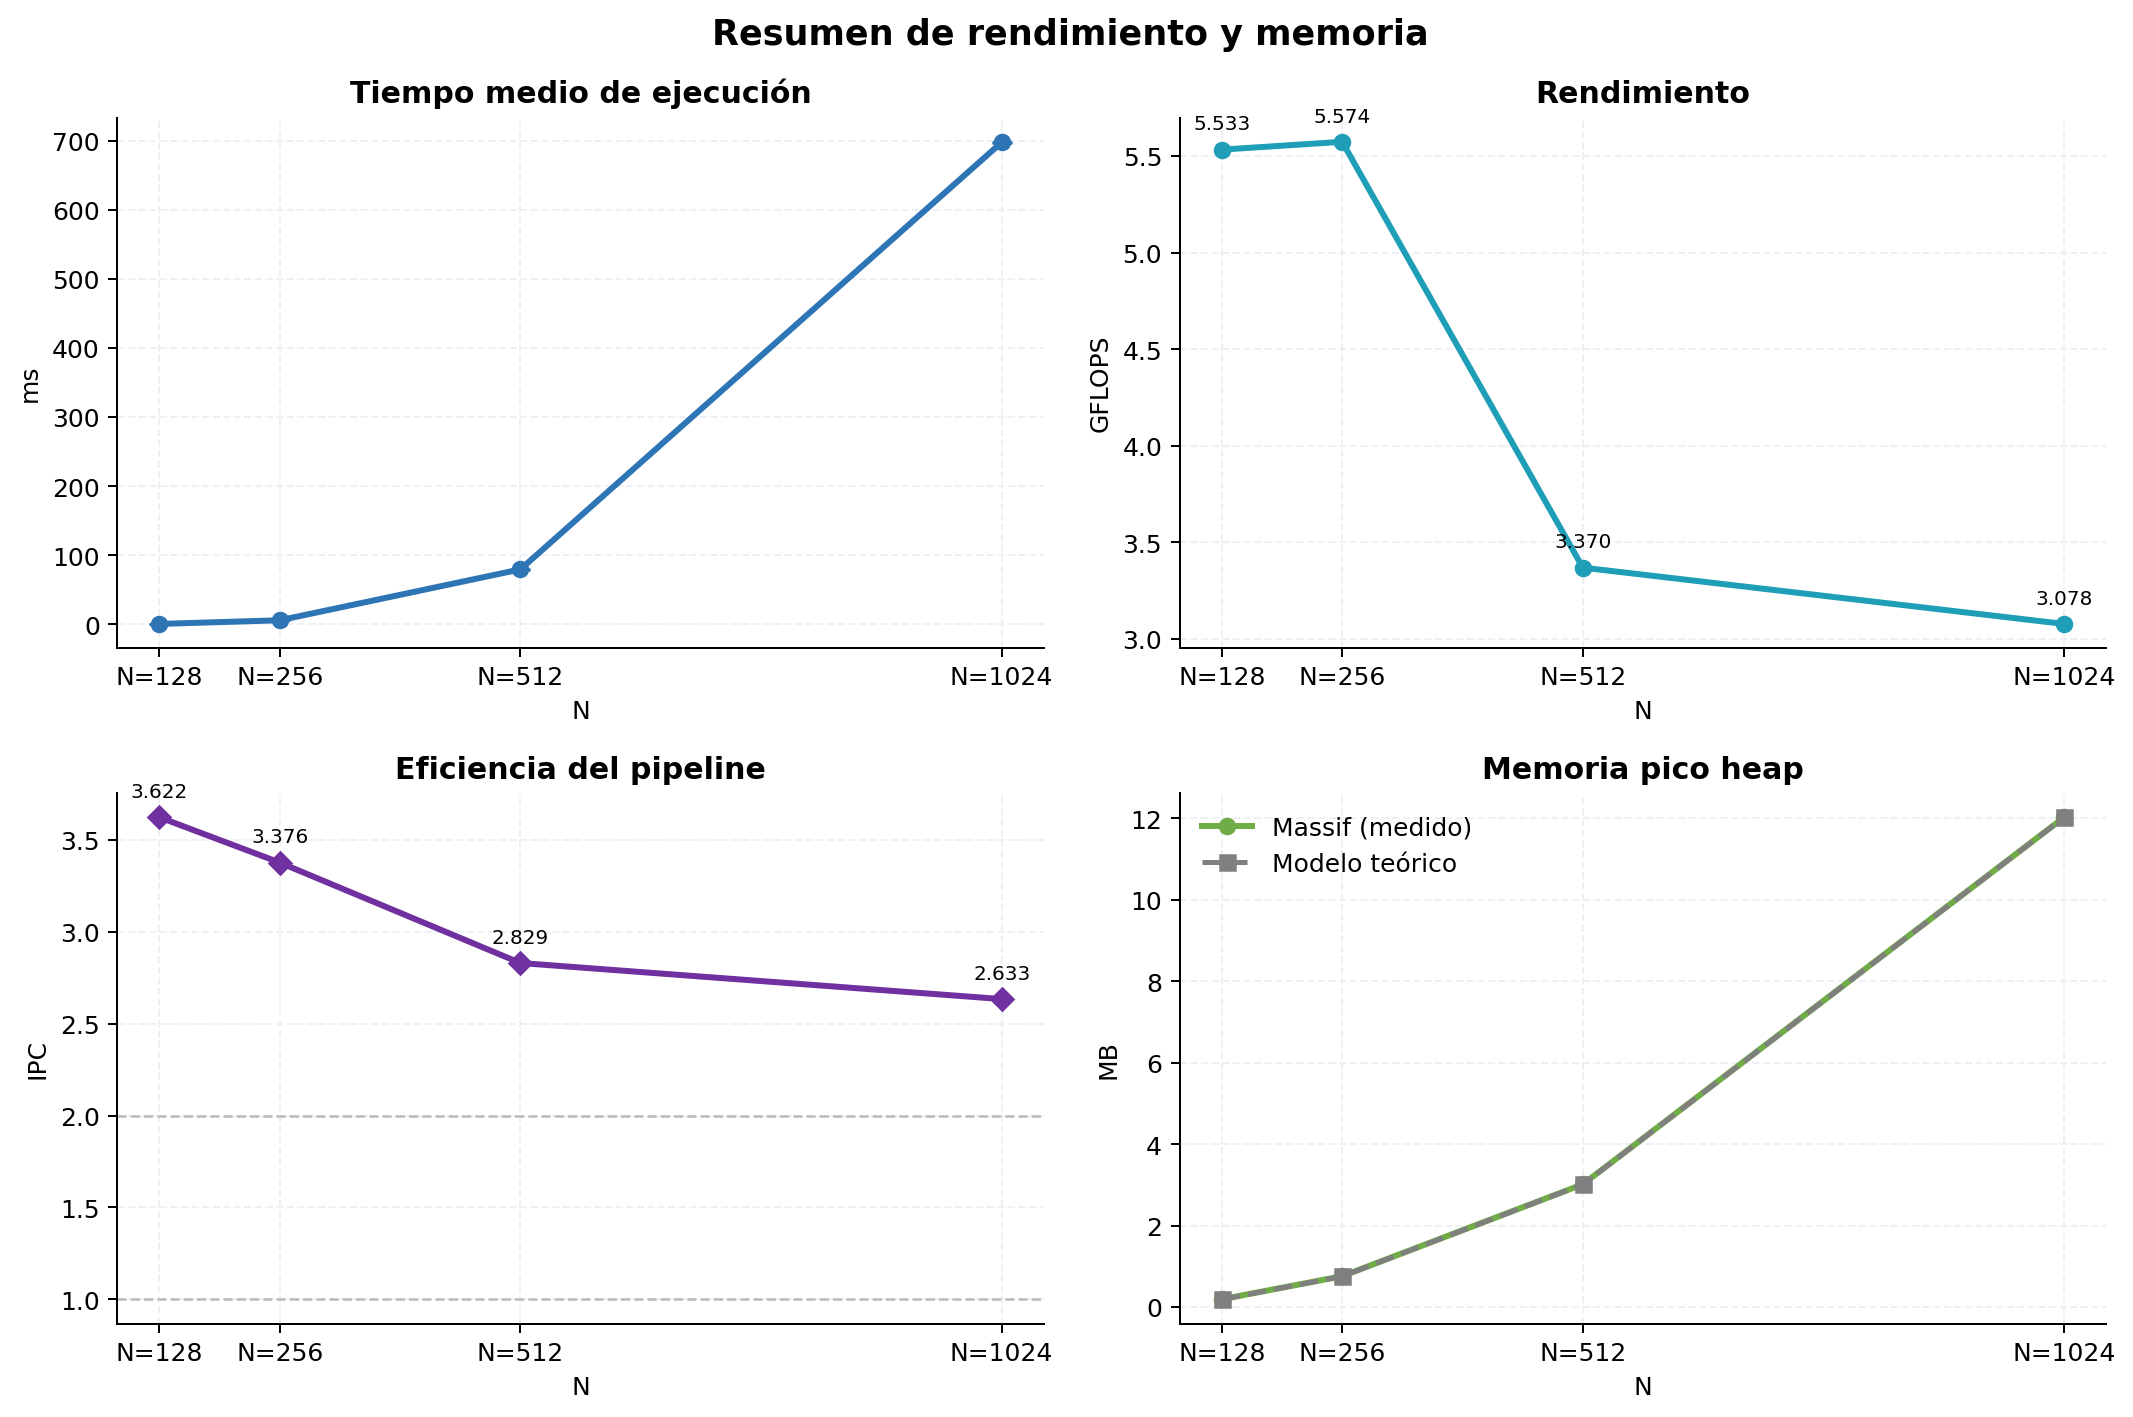
\includegraphics[width=1\textwidth]{images/profiling/01_performance_summary.png}
\caption{Resumen de rendimiento mostrando la caída progresiva de GFLOPS en función de los incrementos en tiempo y en la talla $N$.}
\label{fig:prof_perf}
\end{figure}

\begin{figure}[H]
\centering
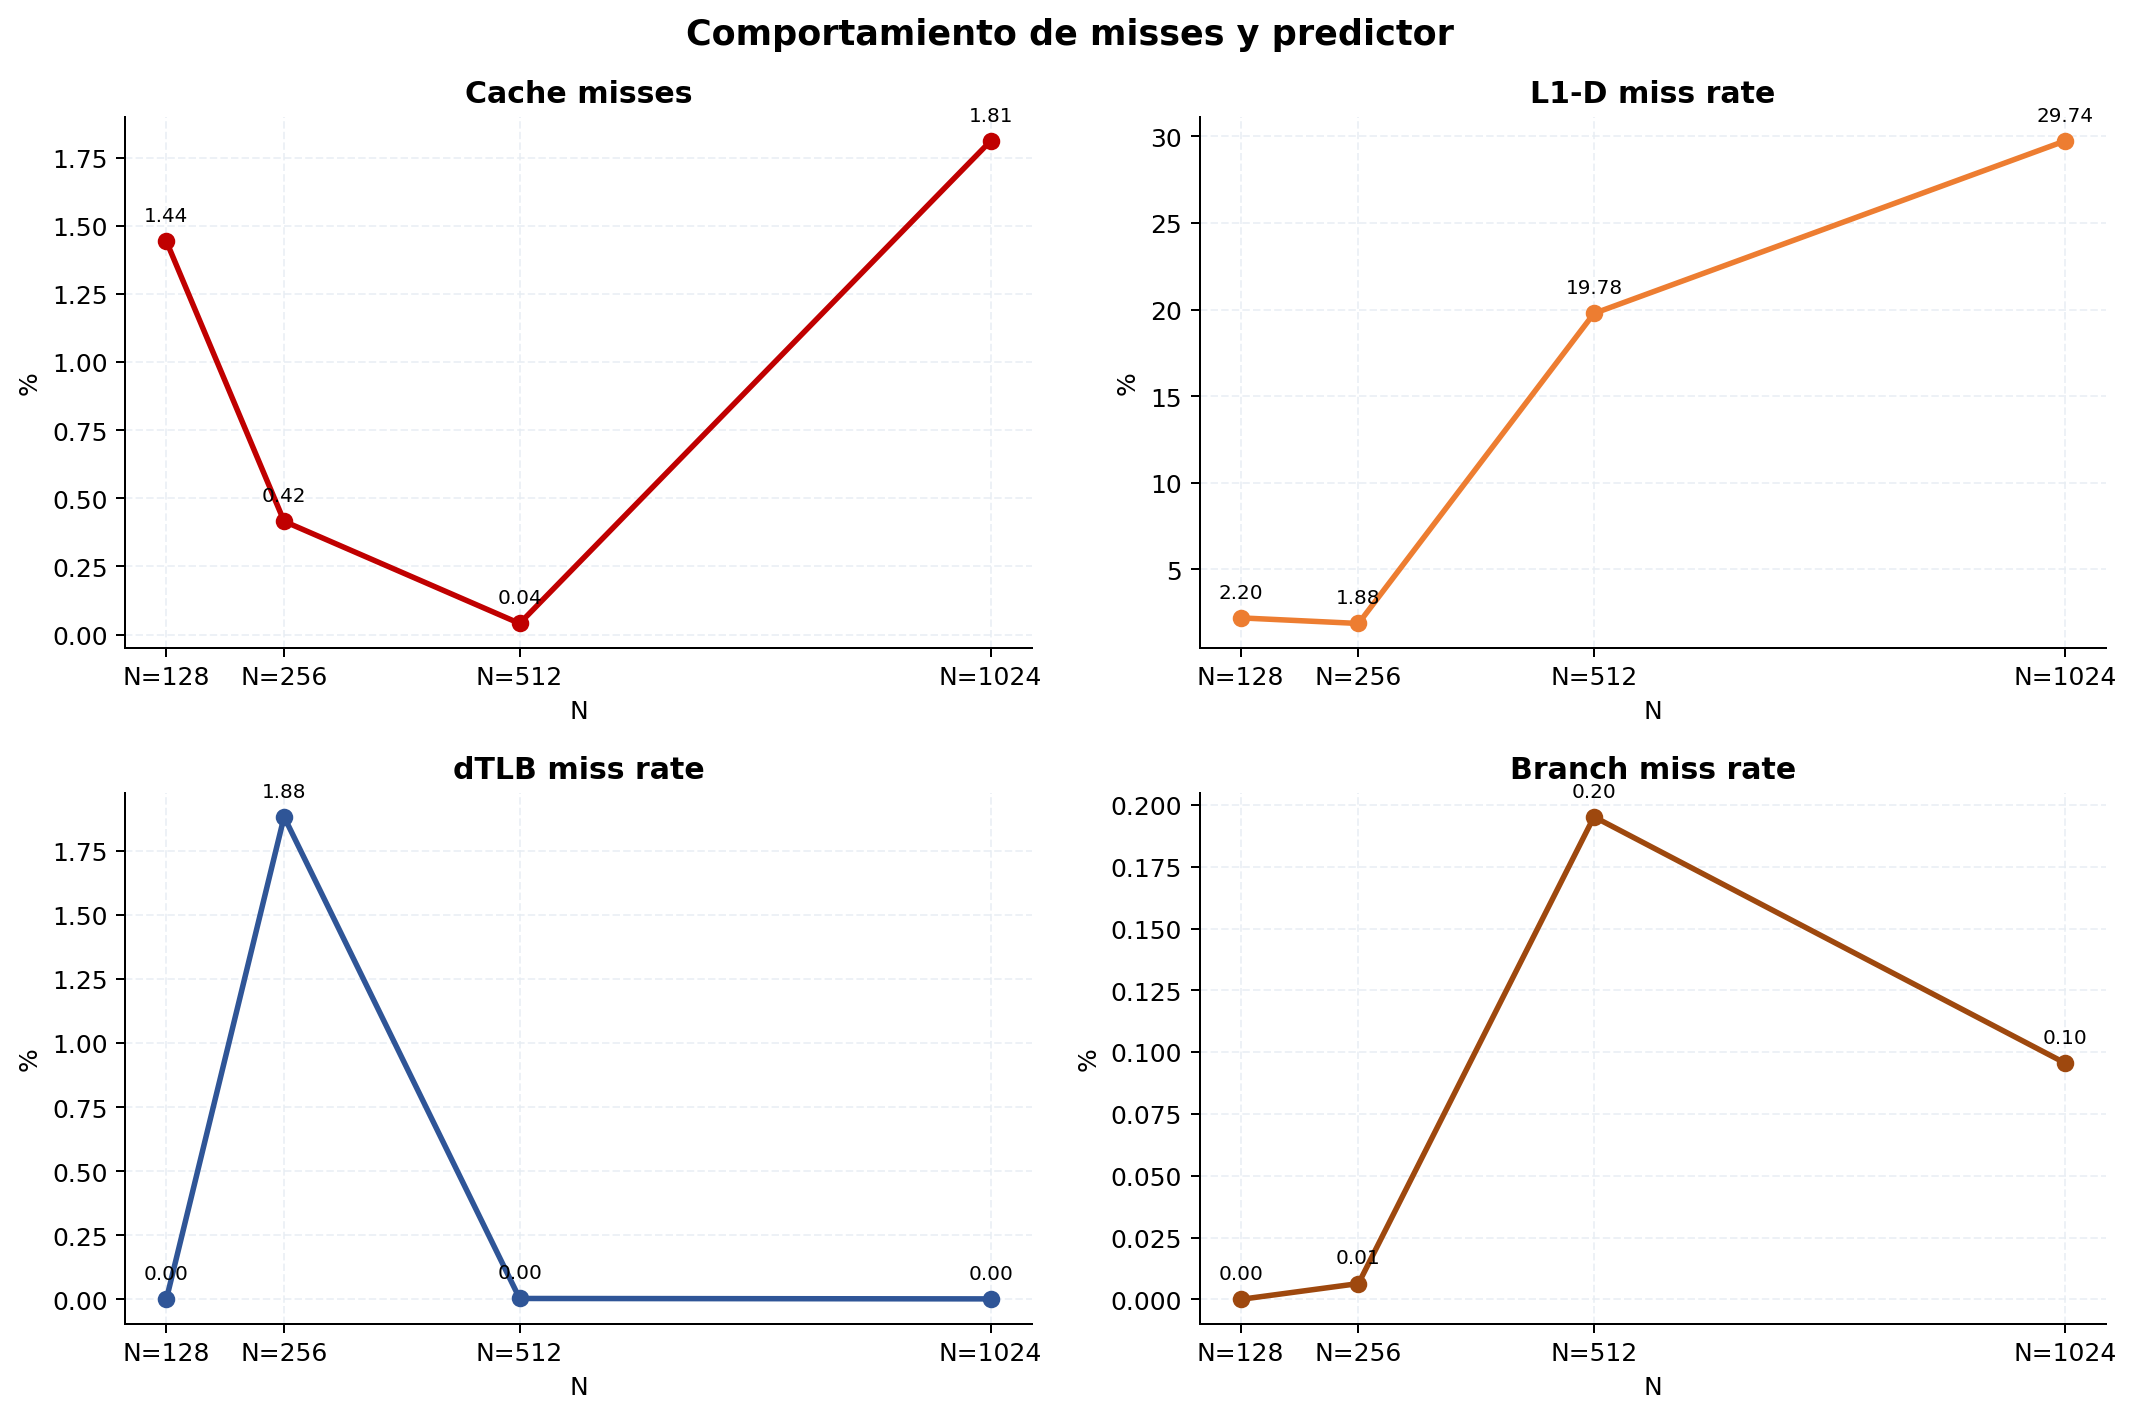
\includegraphics[width=1\textwidth]{images/profiling/02_miss_rates.png}
\caption{Correlación de tasas de fallo, acentuando el incremento en la caché de datos de nivel 1 frente a la estabilidad del predictor de ramas y la dTLB.}
\label{fig:prof_miss}
\end{figure}

Esta degradación tiene tres causas que se pudieron indentificar. La primera es la presión sobre la caché de nivel 1: cuando las matrices son pequeñas ($N=128$), los datos residen prácticamente en caché y la tasa de fallos en L1 es de apenas 2.21\%. Al escalar a $N=1024$, esa tasa asciende a 29.68\%, lo que refleja un patrón de acceso desfavorable. En C, los arreglos bidimensionales se almacenan en orden de filas, de modo que recorrer la segunda matriz por columnas, como exige el producto interior, genera accesos no contiguos en memoria y produce líneas de caché ineficientes.

La segunda causa es la degradación del IPC. Para $N=128$, el procesador logra un IPC de 5.63, aprovechando el paralelismo a nivel de instrucción disponible cuando los datos están en caché. A medida que los fallos de L1 obligan a recurrir a niveles más lentos de la jerarquía de memoria, el pipeline queda en espera y el IPC cae a 2.61 para $N=1024$.

El tercer aspecto relevante es la estabilidad de los demás contadores. Los fallos de predicción de ramas se mantienen por debajo del 0.2\% en todos los casos, lo cual es esperable dado el flujo de control regular de los bucles. Las presiones sobre la TLB tampoco representan un factor limitante, con tasas cercanas a cero en todos los tamaños evaluados. Esto confirma que la caché de datos de nivel 1 es el cuello de botella dominante.

\subsubsection{Uso de memoria dinámica}

El análisis con Valgrind Massif muestra que el consumo de heap escala de forma cuadrática con $N$, pasando de 0.194 MB para $N=128$ hasta 12.027 MB para $N=1024$. Este comportamiento coincide con la estimación teórica esperada: tres matrices de enteros de 32 bits con $N=1024$ requieren aproximadamente $1024 \times 1024 \times 4 \times 3 \approx 12$ MB. La ausencia de fragmentación o metadata excesiva confirma que el gestor de memoria del sistema no introduce sobrecarga anómala, y que cualquier limitante de rendimiento observada se origina en la ejecución del bucle de multiplicación y no en la gestión de memoria dinámica.

\subsubsection{Distribución de accesos a memoria (perf mem / IBS)}

La Figura~\ref{fig:prof_mem} presenta la distribución de los accesos de carga entre los niveles de la jerarquía de memoria, obtenida mediante \texttt{perf mem} con el mecanismo IBS (\textit{Instruction Based Sampling}) del procesador Ryzen 5 7600X. A diferencia de PEBS en arquitecturas Intel, IBS muestrea instrucciones en lugar de eventos de memoria directamente, lo que produce una fracción de muestras no clasificables reportadas como N/A, cuyo porcentaje se indica a la derecha de cada barra.

\begin{figure}[H]
\centering
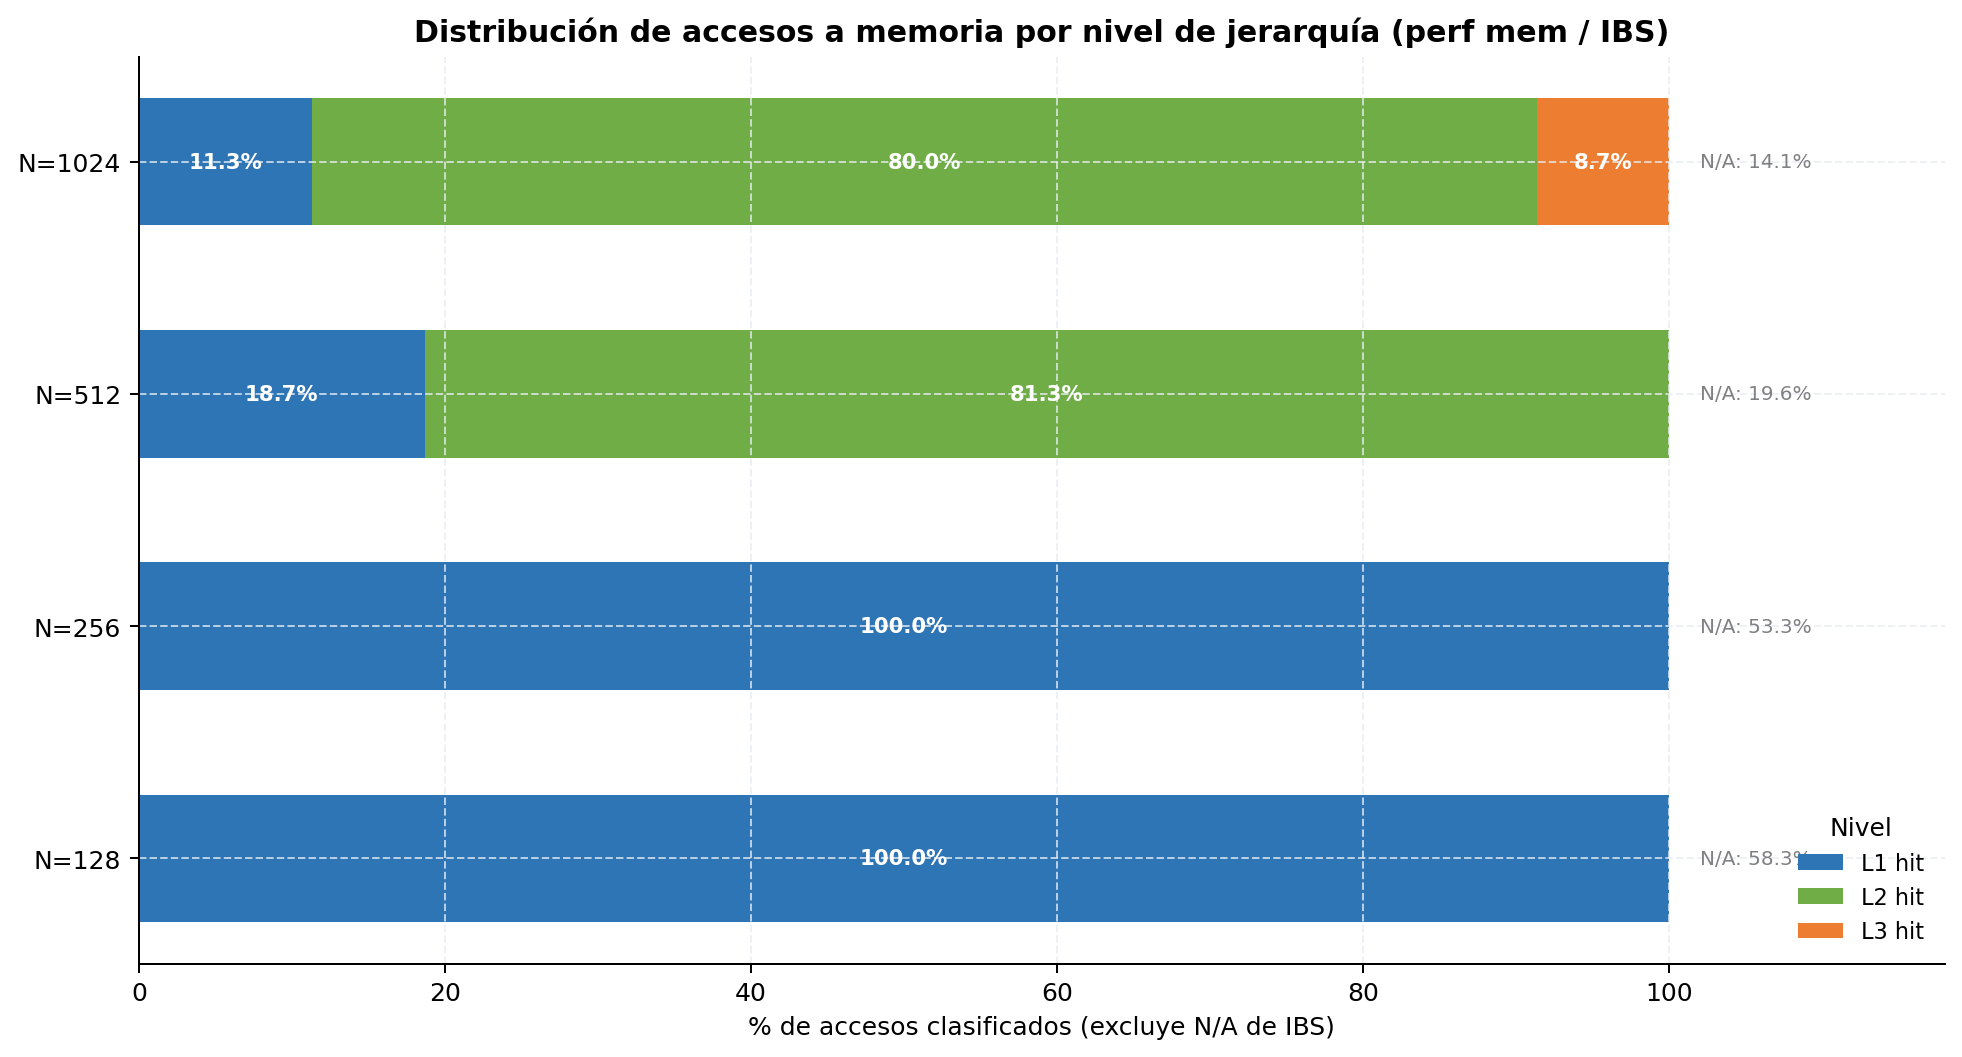
\includegraphics[width=0.9\textwidth]{images/profiling/06_mem_access_distribution.png}
\caption{Distribución porcentual de accesos de carga clasificados por nivel de la jerarquía de memoria (perf mem / IBS). El porcentaje N/A indica muestras no clasificables por el mecanismo IBS de AMD Zen 4.}
\label{fig:prof_mem}
\end{figure}

Para los tamaños pequeños ($N=128$ y $N=256$), la totalidad de los accesos clasificados se sirve desde L1, lo que refleja que las matrices caben activamente en caché durante la ejecución y el hardware logra satisfacer la mayoría de las cargas sin escalar a niveles superiores. A partir de $N=512$ el comportamiento cambia: el 81.3\% de los accesos clasificados provienen de L2, y L1 retiene apenas el 18.7\% restante. Esta transición indica que las matrices superan la capacidad efectiva de la caché L1 y el hardware debe recurrir al siguiente nivel de la jerarquía para servir la mayor parte de las cargas.

Para $N=1024$, el patrón se consolida con un 80.0\% de accesos desde L2, un 11.3\% que aún se resuelve en L1 y un 8.7\% que requiere L3. La ausencia de accesos a RAM principal en los accesos clasificados, combinada con el 14.1\% de N/A, es consistente con el comportamiento de IBS en Zen 4: los accesos con latencias muy altas tienen mayor probabilidad de quedar sin clasificar al no completarse dentro de la ventana de muestreo. El resultado central es que el grueso de las cargas del algoritmo de multiplicación de matrices recae sobre L2 para matrices medianas y grandes, lo que concuerda con la tasa de L1 miss del 29.68\% reportada por \texttt{perf stat} para $N=1024$. Los accesos que fallan en L1 son servidos mayoritariamente desde L2, lo que implica latencias de entre 5 y 12 ciclos adicionales por acceso. Dado que el bucle interno ejecuta $n^2$ accesos sobre la segunda matriz con un patrón de stride columnar, esta penalidad acumulada explica directamente la caída del IPC de 5.63 a 2.61 observada al escalar de $N=128$ a $N=1024$.